\documentclass{standalone}
\usepackage{tikz}
\usetikzlibrary{patterns, positioning}
\usepackage[sfdefault]{ClearSans} %% option 'sfdefault' activates Clear Sans as the default text font
\usepackage[T1]{fontenc}

\begin{document}
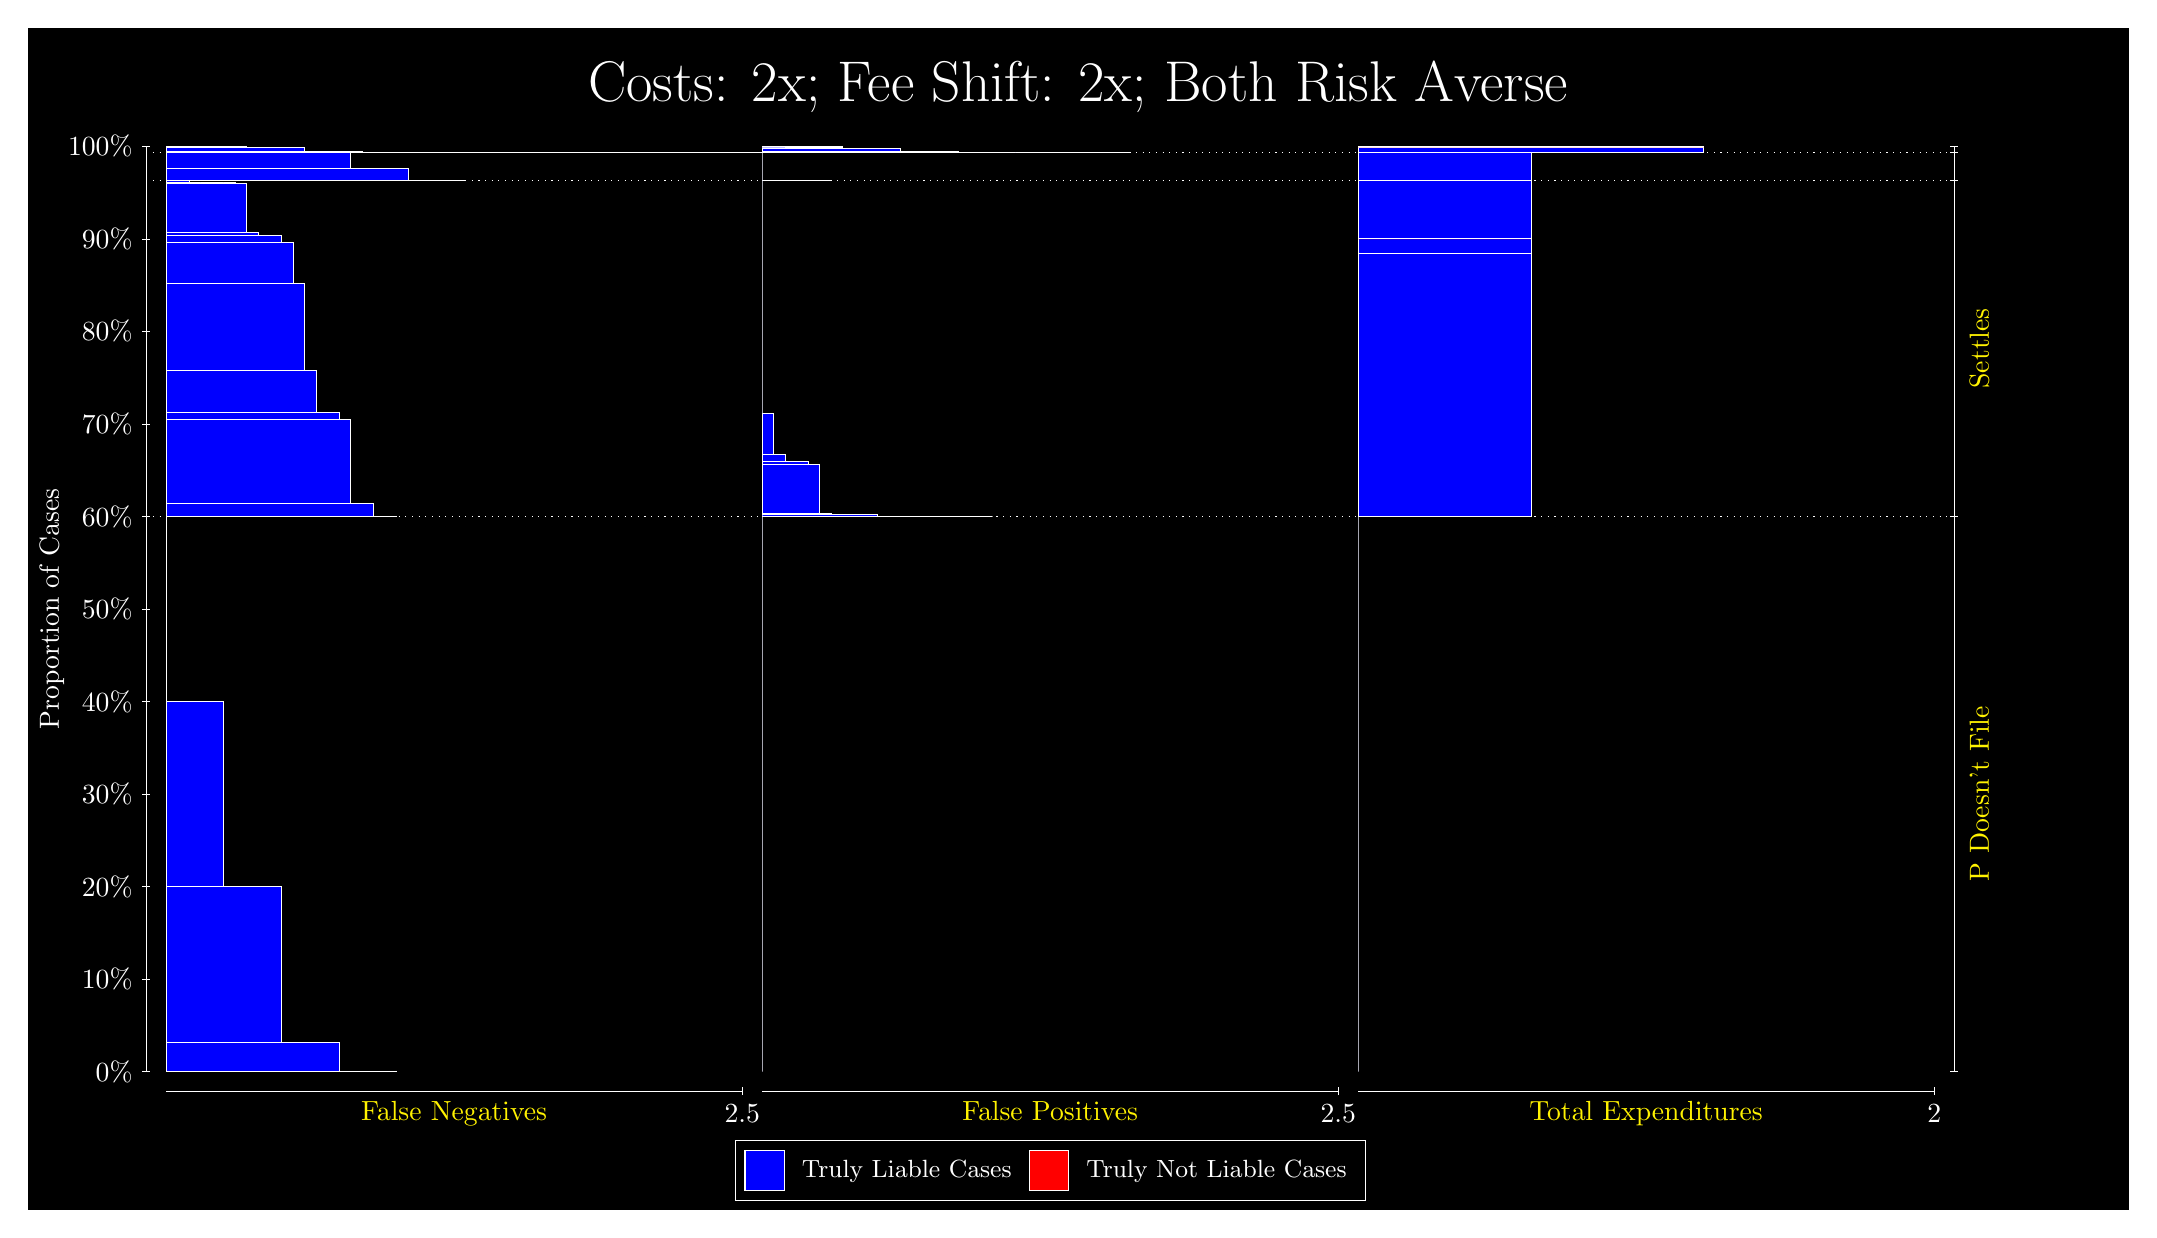
\begin{tikzpicture}
\draw[fill=black] (0,0) rectangle (26.667,15);
\draw[text=white] (0,13.5) rectangle (26.667,15) node[midway] {\huge Costs: 2x; Fee Shift: 2x; Both Risk Averse};
\draw[white, very thin] (1.5,1.75) -- (1.5,13.5);
\node[rotate=90, text=white, anchor=center] at (0.3, 7.625) {Proportion of Cases};
\draw[white, very thin] (1.45,1.75) -- (1.55,1.75);
\node[text=white, anchor=east] at (1.45, 1.75) {0\%};
\draw[white, very thin] (1.45,2.925) -- (1.55,2.925);
\node[text=white, anchor=east] at (1.45, 2.925) {10\%};
\draw[white, very thin] (1.45,4.1) -- (1.55,4.1);
\node[text=white, anchor=east] at (1.45, 4.1) {20\%};
\draw[white, very thin] (1.45,5.275) -- (1.55,5.275);
\node[text=white, anchor=east] at (1.45, 5.275) {30\%};
\draw[white, very thin] (1.45,6.45) -- (1.55,6.45);
\node[text=white, anchor=east] at (1.45, 6.45) {40\%};
\draw[white, very thin] (1.45,7.625) -- (1.55,7.625);
\node[text=white, anchor=east] at (1.45, 7.625) {50\%};
\draw[white, very thin] (1.45,8.8) -- (1.55,8.8);
\node[text=white, anchor=east] at (1.45, 8.8) {60\%};
\draw[white, very thin] (1.45,9.975) -- (1.55,9.975);
\node[text=white, anchor=east] at (1.45, 9.975) {70\%};
\draw[white, very thin] (1.45,11.15) -- (1.55,11.15);
\node[text=white, anchor=east] at (1.45, 11.15) {80\%};
\draw[white, very thin] (1.45,12.325) -- (1.55,12.325);
\node[text=white, anchor=east] at (1.45, 12.325) {90\%};
\draw[white, very thin] (1.45,13.5) -- (1.55,13.5);
\node[text=white, anchor=east] at (1.45, 13.5) {100\%};

\draw[white, very thin] (24.457,1.75) -- (24.457,13.5);
\draw[white, very thin] (24.407,1.75) -- (24.507,1.75);
\node[anchor=west] at (24.407, 1.75) {};
\draw[white, very thin] (24.407,8.8012) -- (24.507,8.8012);
\node[anchor=west] at (24.407, 8.8012) {};
\draw[white, very thin] (24.407,13.067) -- (24.507,13.067);
\node[anchor=west] at (24.407, 13.067) {};
\draw[white, very thin] (24.407,13.422) -- (24.507,13.422);
\node[anchor=west] at (24.407, 13.422) {};
\draw[white, very thin] (24.407,13.5) -- (24.507,13.5);
\node[anchor=west] at (24.407, 13.5) {};

\draw[white, very thin, fill=blue] (1.75,1.75) rectangle (4.6775,1.7538);
\draw[white, very thin, fill=blue] (1.75,1.7538) rectangle (3.9457,2.1271);
\draw[white, very thin, fill=blue] (1.75,2.1271) rectangle (3.2138,4.1043);
\draw[white, very thin, fill=blue] (1.75,4.1043) rectangle (2.4819,6.4512);
\draw[white, very thin, fill=red] (1.75,6.4512) rectangle (1.75,6.4512);
\draw[white, very thin, fill=blue] (1.75,6.4512) rectangle (1.75,8.8012);
\draw[white, very thin, fill=blue] (1.75,8.8012) rectangle (4.6775,8.8014);
\draw[white, very thin, fill=blue] (1.75,8.8014) rectangle (4.3848,8.9678);
\draw[white, very thin, fill=blue] (1.75,8.9678) rectangle (4.092,10.036);
\draw[white, very thin, fill=blue] (1.75,10.036) rectangle (3.9457,10.128);
\draw[white, very thin, fill=blue] (1.75,10.128) rectangle (3.6529,10.662);
\draw[white, very thin, fill=blue] (1.75,10.662) rectangle (3.5065,11.761);
\draw[white, very thin, fill=blue] (1.75,11.761) rectangle (3.3602,12.28);
\draw[white, very thin, fill=blue] (1.75,12.28) rectangle (3.2138,12.371);
\draw[white, very thin, fill=blue] (1.75,12.371) rectangle (2.921,12.41);
\draw[white, very thin, fill=blue] (1.75,12.41) rectangle (2.7746,13.026);
\draw[white, very thin, fill=blue] (1.75,13.026) rectangle (2.6283,13.046);
\draw[white, very thin, fill=blue] (1.75,13.046) rectangle (2.4819,13.046);
\draw[white, very thin, fill=blue] (1.75,13.046) rectangle (2.1891,13.046);
\draw[white, very thin, fill=blue] (1.75,13.046) rectangle (2.0428,13.067);
\draw[white, very thin, fill=blue] (1.75,13.067) rectangle (1.8964,13.067);
\draw[white, very thin, fill=red] (1.75,13.067) rectangle (1.75,13.067);
\draw[white, very thin, fill=blue] (1.75,13.067) rectangle (1.75,13.067);
\draw[white, very thin, fill=blue] (1.75,13.067) rectangle (5.5558,13.069);
\draw[white, very thin, fill=blue] (1.75,13.069) rectangle (4.8239,13.227);
\draw[white, very thin, fill=blue] (1.75,13.227) rectangle (4.092,13.42);
\draw[white, very thin, fill=blue] (1.75,13.42) rectangle (3.3602,13.422);
\draw[white, very thin, fill=blue] (1.75,13.422) rectangle (2.6283,13.422);
\draw[white, very thin, fill=red] (1.75,13.422) rectangle (1.75,13.422);
\draw[white, very thin, fill=blue] (1.75,13.422) rectangle (9.9471,13.422);
\draw[white, very thin, fill=blue] (1.75,13.422) rectangle (9.2152,13.422);
\draw[white, very thin, fill=blue] (1.75,13.422) rectangle (8.4834,13.424);
\draw[white, very thin, fill=blue] (1.75,13.424) rectangle (7.7515,13.426);
\draw[white, very thin, fill=blue] (1.75,13.426) rectangle (7.0196,13.426);
\draw[white, very thin, fill=blue] (1.75,13.426) rectangle (6.2877,13.426);
\draw[white, very thin, fill=blue] (1.75,13.426) rectangle (5.7022,13.426);
\draw[white, very thin, fill=blue] (1.75,13.426) rectangle (5.5558,13.426);
\draw[white, very thin, fill=blue] (1.75,13.426) rectangle (4.9703,13.426);
\draw[white, very thin, fill=blue] (1.75,13.426) rectangle (4.2384,13.443);
\draw[white, very thin, fill=blue] (1.75,13.443) rectangle (3.5065,13.484);
\draw[white, very thin, fill=blue] (1.75,13.484) rectangle (2.7746,13.5);
\draw[white, very thin, fill=blue] (1.75,13.5) rectangle (2.0428,13.5);
\draw[white, very thin, fill=red] (1.75,13.5) rectangle (1.75,13.5);
\draw[white, very thin, fill=blue] (1.75,13.5) rectangle (1.75,13.5);
\draw[white, very thin, fill=red] (9.3189,1.75) rectangle (9.3189,1.75);
\draw[white, very thin, fill=blue] (9.3189,1.75) rectangle (9.3189,8.8012);
\draw[white, very thin, fill=red] (9.3189,8.8012) rectangle (12.246,8.8012);
\draw[white, very thin, fill=blue] (9.3189,8.8012) rectangle (12.246,8.8012);
\draw[white, very thin, fill=red] (9.3189,8.8012) rectangle (11.661,8.8012);
\draw[white, very thin, fill=blue] (9.3189,8.8012) rectangle (11.661,8.8012);
\draw[white, very thin, fill=blue] (9.3189,8.8012) rectangle (11.515,8.8012);
\draw[white, very thin, fill=red] (9.3189,8.8012) rectangle (11.368,8.8012);
\draw[white, very thin, fill=blue] (9.3189,8.8012) rectangle (11.368,8.8012);
\draw[white, very thin, fill=red] (9.3189,8.8012) rectangle (11.075,8.8012);
\draw[white, very thin, fill=blue] (9.3189,8.8012) rectangle (11.075,8.8012);
\draw[white, very thin, fill=blue] (9.3189,8.8012) rectangle (10.929,8.8012);
\draw[white, very thin, fill=blue] (9.3189,8.8012) rectangle (10.783,8.8215);
\draw[white, very thin, fill=blue] (9.3189,8.8215) rectangle (10.636,8.8215);
\draw[white, very thin, fill=blue] (9.3189,8.8215) rectangle (10.344,8.8217);
\draw[white, very thin, fill=blue] (9.3189,8.8217) rectangle (10.197,8.8416);
\draw[white, very thin, fill=blue] (9.3189,8.8416) rectangle (10.051,9.4575);
\draw[white, very thin, fill=blue] (9.3189,9.4575) rectangle (9.9044,9.497);
\draw[white, very thin, fill=blue] (9.3189,9.497) rectangle (9.6116,9.588);
\draw[white, very thin, fill=blue] (9.3189,9.588) rectangle (9.4652,10.106);
\draw[white, very thin, fill=blue] (9.3189,10.106) rectangle (9.3189,13.067);
\draw[white, very thin, fill=red] (9.3189,13.067) rectangle (10.197,13.067);
\draw[white, very thin, fill=blue] (9.3189,13.067) rectangle (10.197,13.067);
\draw[white, very thin, fill=blue] (9.3189,13.067) rectangle (9.4652,13.069);
\draw[white, very thin, fill=blue] (9.3189,13.069) rectangle (9.3189,13.422);
\draw[white, very thin, fill=red] (9.3189,13.422) rectangle (14.003,13.422);
\draw[white, very thin, fill=blue] (9.3189,13.422) rectangle (14.003,13.422);
\draw[white, very thin, fill=red] (9.3189,13.422) rectangle (13.271,13.422);
\draw[white, very thin, fill=blue] (9.3189,13.422) rectangle (13.271,13.422);
\draw[white, very thin, fill=red] (9.3189,13.422) rectangle (12.539,13.422);
\draw[white, very thin, fill=blue] (9.3189,13.422) rectangle (12.539,13.422);
\draw[white, very thin, fill=blue] (9.3189,13.422) rectangle (11.807,13.439);
\draw[white, very thin, fill=red] (9.3189,13.439) rectangle (11.807,13.439);
\draw[white, very thin, fill=blue] (9.3189,13.439) rectangle (11.807,13.439);
\draw[white, very thin, fill=blue] (9.3189,13.439) rectangle (11.075,13.479);
\draw[white, very thin, fill=blue] (9.3189,13.479) rectangle (11.075,13.479);
\draw[white, very thin, fill=blue] (9.3189,13.479) rectangle (10.344,13.494);
\draw[white, very thin, fill=blue] (9.3189,13.494) rectangle (10.344,13.496);
\draw[white, very thin, fill=blue] (9.3189,13.496) rectangle (9.6116,13.496);
\draw[white, very thin, fill=blue] (9.3189,13.496) rectangle (9.6116,13.496);
\draw[white, very thin, fill=red] (9.3189,13.496) rectangle (9.3189,13.496);
\draw[white, very thin, fill=blue] (9.3189,13.496) rectangle (9.3189,13.5);
\draw[white, very thin, fill=red] (16.888,1.75) rectangle (16.888,1.75);
\draw[white, very thin, fill=blue] (16.888,1.75) rectangle (16.888,8.8012);
\draw[white, very thin, fill=red] (16.888,8.8012) rectangle (19.083,8.8012);
\draw[white, very thin, fill=blue] (16.888,8.8012) rectangle (19.083,12.144);
\draw[white, very thin, fill=red] (16.888,12.144) rectangle (19.083,12.144);
\draw[white, very thin, fill=blue] (16.888,12.144) rectangle (19.083,12.327);
\draw[white, very thin, fill=red] (16.888,12.327) rectangle (19.083,12.327);
\draw[white, very thin, fill=blue] (16.888,12.327) rectangle (19.083,13.067);
\draw[white, very thin, fill=red] (16.888,13.067) rectangle (19.083,13.067);
\draw[white, very thin, fill=blue] (16.888,13.067) rectangle (19.083,13.422);
\draw[white, very thin, fill=red] (16.888,13.422) rectangle (21.279,13.422);
\draw[white, very thin, fill=blue] (16.888,13.422) rectangle (21.279,13.494);
\draw[white, very thin, fill=red] (16.888,13.494) rectangle (21.279,13.494);
\draw[white, very thin, fill=blue] (16.888,13.494) rectangle (21.279,13.496);
\draw[white, very thin, fill=red] (16.888,13.496) rectangle (21.279,13.496);
\draw[white, very thin, fill=blue] (16.888,13.496) rectangle (21.279,13.5);
\draw[white, dotted] (1.5,8.8012) -- (24.457,8.8012);
\draw[white, dotted] (1.5,13.067) -- (24.457,13.067);
\draw[white, dotted] (1.5,13.422) -- (24.457,13.422);
\draw[white, very thin] (1.75,1.5) -- (9.0689,1.5);
\node[text=yellow, anchor=north] at (5.4094, 1.5) {False Negatives};
\draw[white, very thin] (9.0689,1.45) -- (9.0689,1.55);
\node[text=white, anchor=north] at (9.0689, 1.45) {2.5};

\draw[white, very thin] (9.3189,1.5) -- (16.638,1.5);
\node[text=yellow, anchor=north] at (12.978, 1.5) {False Positives};
\draw[white, very thin] (16.638,1.45) -- (16.638,1.55);
\node[text=white, anchor=north] at (16.638, 1.45) {2.5};

\draw[white, very thin] (16.888,1.5) -- (24.207,1.5);
\node[text=yellow, anchor=north] at (20.547, 1.5) {Total Expenditures};
\draw[white, very thin] (24.207,1.45) -- (24.207,1.55);
\node[text=white, anchor=north] at (24.207, 1.45) {2};

\node[text=yellow, centered, rotate=90] at (24.777, 5.2756) {P Doesn't File};
\node[text=yellow, centered, rotate=90] at (24.777, 10.934) {Settles};



\draw (12.978300999999998,1.5) node[draw=none] (baseCoordinate) {};
\begin{scope}[align=center]
        \matrix[scale=0.5, draw=white, below=0.5cm of baseCoordinate, nodes={draw}, column sep=0.1cm]{
            \node[rectangle, draw, minimum width=0.5cm, minimum height=0.5cm, fill=blue] {}; &
            \node[draw=none, font=\small, text=white] (B) {Truly Liable Cases}; &
            \node[rectangle, draw, minimum width=0.5cm, minimum height=0.5cm, fill=red] {}; &
            \node[draw=none, font=\small, text=white] (B) {Truly Not Liable Cases}; \\
            };
\end{scope}

\end{tikzpicture}
\end{document}